\documentclass[aspectratio=169]{beamer}
\usepackage[utf8]{inputenc}

% design
\usetheme{CambridgeUS}
\usecolortheme{beaver}
\setbeamertemplate{itemize items}[square]
\usenavigationsymbolstemplate{\beamertemplatenavigationsymbolsempty}
\definecolor{darkred}{rgb}{0.8,0,0}
\colorlet{grey1}{gray!10!white} % I think = RGB 0.95 0.95 0.95
\colorlet{grey2}{gray!60!white} % I think = RGB 0.7 0.7 0.7
\setbeamercolor{structure}{fg=darkred}
\setbeamertemplate{enumerate item}{\insertenumlabel.}
\setbeamertemplate{itemize item}{$\blacktriangleright$}
\setlength{\tabcolsep}{12pt}
\setbeamercolor{block title}{fg=darkred}

% bibliography
%\usepackage[backend=biber, style=authortitle]{biblatex}
\usepackage{natbib}
\usepackage{har2nat}
\bibliographystyle{unsrt}
%\addbibresource{../../smc.bib}
\usepackage{bibentry}
\nobibliography*

% tikz
\usepackage{tikz}
\usetikzlibrary{positioning}

% maths
\usepackage{amsmath}
\usepackage{amssymb}
\usepackage{amsfonts}
\usepackage{amsthm}
\theoremstyle{definition}
\newtheorem{defn}{Definition}

% useful math symbols
\newcommand{\PR}{\mathbb{P}}
\newcommand{\E}{\mathbb{E}}
\newcommand{\V}{\operatorname{Var}}
\newcommand{\eqdist}{\overset{d}{=}}
\newcommand{\I}[1]{\mathbb{I}\{#1\}}
\newcommand{\Ntoinfty}{\overset{N\to\infty}{\longrightarrow}}
\newcommand{\limNtoinfty}{\underset{N\to\infty}{\lim}}
\newcommand\indep{\protect\mathpalette{\protect\independenT}{\perp}}
\def\independenT#1#2{\mathrel{\rlap{$#1#2$}\mkern2mu{#1#2}}}

% distributions
\newcommand{\N}{\mathcal{N}}
\newcommand{\Cat}{\operatorname{Categorical}}
\newcommand{\Unif}{\operatorname{Uniform}}
\newcommand{\Mn}{\operatorname{Multinomial}}
\newcommand{\Bin}{\operatorname{Binomial}}

% project-specific commands
\newcommand{\F}{\mathcal{F}_{t-1}}
\newcommand{\vt}[2][t]{\nu_{#1}^{(#2)}}
%\newcommand{\vt}[1]{v_{#1}}
\newcommand{\wt}[2][t]{w_{#1}^{(#2)}}
%\newcommand{\wt}[1]{w_{#1}}
%\newcommand{\wbar}[2][t]{\bar{w}_{#1}^{(#2)}}
%\newcommand{\vttilde}[2][t]{\tilde{v}_{#1}^{(#2)}}
\newcommand{\Et}{\mathbb{E}_{t}}

\title[]{Asymptotic genealogies of non-neutral populations}
\author[Suzie Brown]{\textbf{Suzie Brown} \\[5pt] University of Warwick, U.K. \\ with Paul Jenkins, Adam Johansen \& Jere Koskela}
\date{13 May 2021} 

\begin{document}
\begin{frame}
\maketitle
\end{frame}


\begin{frame}{Interacting particle system}
\begin{itemize}
\item Constant population size $N$
\item ``Genotype'' $X_t^{(i)} \in \mathcal{X} \subseteq \mathbb{R}^d$
\item Initial genotypes $X_0 \sim \mu$
\end{itemize}
\end{frame}


\begin{frame}{Interacting particle system}
\begin{center}
\resizebox{0.95\textwidth}{!}{%
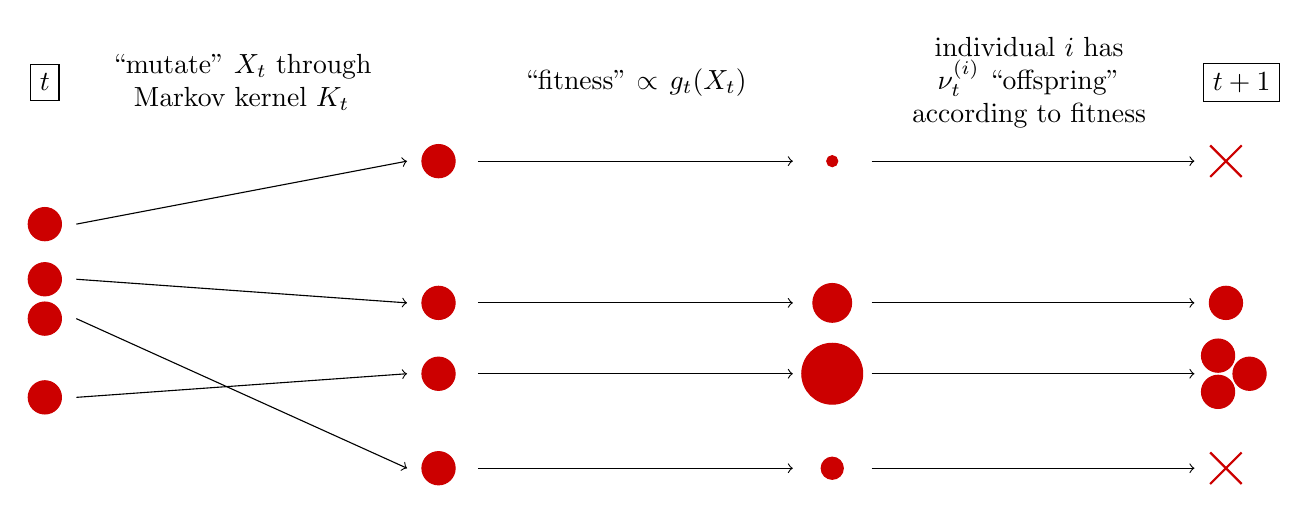
\begin{tikzpicture}
\filldraw[darkred] (0,0) circle (6pt);
\filldraw[darkred] (0,1) circle (6pt);
\filldraw[darkred] (0,1.5) circle (6pt);
\filldraw[darkred] (0,2.2) circle (6pt);
\node[rectangle, draw=black] at (0,4) {$t$};

\pause

\node[text width = 10em, text centered] at (2.5,4) {{``mutate'' $X_t$ through\\ Markov kernel $K_t$}};

\draw[->] (0.4,2.2) -- (4.6,3);
\draw[->] (0.4,1.5) -- (4.6,1.2);
\draw[->] (0.4,1) -- (4.6,-0.9);
\draw[->] (0.4,0) -- (4.6,0.3);

\filldraw[darkred] (5,0.3) circle (6pt);
\filldraw[darkred] (5,-0.9) circle (6pt);
\filldraw[darkred] (5,1.2) circle (6pt);
\filldraw[darkred] (5,3) circle (6pt);

\pause

\node[text width = 10em, text centered] at (7.5,4) {{``fitness'' $\propto g_t(X_t)$}};

\draw[->] (5.5,3) -- (9.5,3);
\draw[->] (5.5,1.2) -- (9.5,1.2);
\draw[->] (5.5,-0.9) -- (9.5,-0.9);
\draw[->] (5.5,0.3) -- (9.5,0.3);

\filldraw[darkred] (10,0.3) circle (11pt);
\filldraw[darkred] (10,-0.9) circle (4pt);
\filldraw[darkred] (10,1.2) circle (7pt);
\filldraw[darkred] (10,3) circle (2pt);

\pause

\node[text width = 10em, text centered] at (12.5,4) {{individual $i$ has\\ $\nu_t^{(i)}$ ``offspring''\\ according to fitness}};

\draw[->] (10.5,1.2) -- (14.6,1.2);
\draw[->] (10.5,0.3) -- (14.6,0.3);
\draw[->] (10.5,-0.9) -- (14.6,-0.9);
\draw[->] (10.5,3) -- (14.6,3);

\filldraw[darkred] (15.3,0.3) circle (6pt);
\filldraw[darkred] (14.9,0.53) circle (6pt);
\filldraw[darkred] (14.9,0.07) circle (6pt);
\filldraw[darkred] (15,1.2) circle (6pt);

\draw[darkred, thick] (14.8,3.2) -- (15.2, 2.8);
\draw[darkred, thick] (14.8,2.8) -- (15.2, 3.2);
\draw[darkred, thick] (14.8,-0.7) -- (15.2, -1.1);
\draw[darkred, thick] (14.8,-1.1) -- (15.2, -0.7);

\node[rectangle, draw=black] at (15.2,4) {$t+1$};
\end{tikzpicture}
}
\end{center}
\end{frame}


\begin{frame}{Genealogies}
\centering
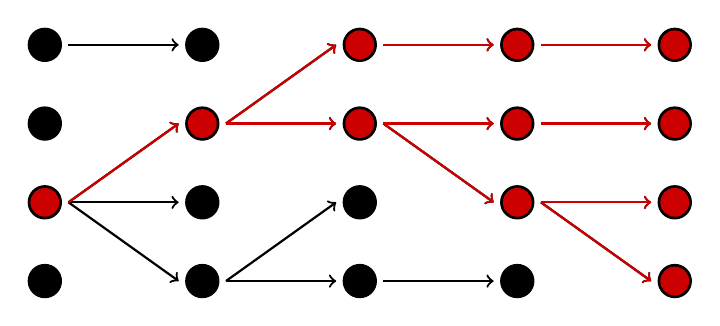
\begin{tikzpicture}
\filldraw (0,0) circle (6pt);
\filldraw (0,-1) circle (6pt);
\filldraw (0,-2) circle (6pt);
\filldraw (0,-3) circle (6pt);

\draw[->, thick] (0.3,0)--(1.7,0);
\draw[->, thick] (0.3,-2)--(1.7,-1);
\draw[->, thick] (0.3,-2)--(1.7,-3);
\draw[->, thick] (0.3,-2)--(1.7,-2);

\filldraw (2,0) circle (6pt);
\filldraw (2,-1) circle (6pt);
\filldraw (2,-2) circle (6pt);
\filldraw (2,-3) circle (6pt);

\pause

\filldraw (4,0) circle (6pt);
\filldraw (4,-1) circle (6pt);
\filldraw (4,-2) circle (6pt);
\filldraw (4,-3) circle (6pt);

\draw[->, thick] (2.3,-1)--(3.7,0);
\draw[->, thick] (2.3,-1)--(3.7,-1);
\draw[->, thick] (2.3,-3)--(3.7,-2);
\draw[->, thick] (2.3,-3)--(3.7,-3);

\filldraw (6,0) circle (6pt);
\filldraw (6,-1) circle (6pt);
\filldraw (6,-2) circle (6pt);
\filldraw (6,-3) circle (6pt);

\filldraw (8,0) circle (6pt);
\filldraw (8,-1) circle (6pt);
\filldraw (8,-2) circle (6pt);
\filldraw (8,-3) circle (6pt);

\draw[->, thick] (4.3,0)--(5.7,0);
\draw[->, thick] (4.3,-1)--(5.7,-1);
\draw[->, thick] (4.3,-1)--(5.7,-2);
\draw[->, thick] (4.3,-3)--(5.7,-3);

\draw[->, thick] (6.3,0)--(7.7,0);
\draw[->, thick] (6.3,-1)--(7.7,-1);
\draw[->, thick] (6.3,-2)--(7.7,-2);
\draw[->, thick] (6.3,-2)--(7.7,-3);

\pause

\filldraw[darkred] (8,0) circle (5pt);
\filldraw[darkred] (6,0) circle (5pt);
\filldraw[darkred] (4,0) circle (5pt);
\filldraw[darkred] (2,-1) circle (5pt);
\filldraw[darkred] (0,-2) circle (5pt);

\draw[->, thick, darkred] (0.3,-2)--(1.7,-1);
\draw[->, thick, darkred] (2.3,-1)--(3.7,0);
\draw[->, thick, darkred] (4.3,0)--(5.7,0);
\draw[->, thick, darkred] (6.3,0)--(7.7,0);

\filldraw[darkred] (4,-1) circle (5pt);
\filldraw[darkred] (6,-1) circle (5pt);
\filldraw[darkred] (8,-1) circle (5pt);
\filldraw[darkred] (6,-2) circle (5pt);
\filldraw[darkred] (8,-2) circle (5pt);
\filldraw[darkred] (8,-3) circle (5pt);

\draw[->, thick, darkred] (2.3,-1)--(3.7,-1);
\draw[->, thick, darkred] (4.3,-1)--(5.7,-1);
\draw[->, thick, darkred] (4.3,-1)--(5.7,-2);
\draw[->, thick, darkred] (6.3,-1)--(7.7,-1);
\draw[->, thick, darkred] (6.3,-2)--(7.7,-2);
\draw[->, thick, darkred] (6.3,-2)--(7.7,-3);
\end{tikzpicture}
\end{frame}


\begin{frame}{Genealogies}
\centering
\begin{tikzpicture}
\draw[dotted] (0,-4.5)--(0,0.5);
\draw[dotted] (2,-4.5)--(2,0.5);
\draw[dotted] (4,-4.5)--(4,0.5);
\draw[dotted] (6,-4.5)--(6,0.5);
\draw[dotted] (8,-4.5)--(8,0.5);

\draw[thick, darkred] (0,-1)--(2,-1);
\draw[thick, darkred] (2,0)--(2,-2);
\draw[thick, darkred] (2,0)--(8,0);
\draw[thick, darkred] (2,-2)--(4,-2);
\draw[thick, darkred] (4,-3)--(4,-1);
\draw[thick, darkred] (4,-1)--(8,-1);
\draw[thick, darkred] (4,-3)--(6,-3);
\draw[thick, darkred] (6,-2)--(6,-4);
\draw[thick, darkred] (6,-2)--(8,-2);
\draw[thick, darkred] (6,-4)--(8,-4);
\end{tikzpicture}
\end{frame}


\begin{frame}{Kingman's $n$-coalescent}%\footnote[frame]{Kingman 1982}}
\begin{columns}
\begin{column}{0.45\textwidth}
\begin{itemize}
\item Continuous-time Markov chain on the space of partitions of $\{1,\dots,n\}$
\item Single pair mergers only
\item Each pair merges independently at rate 1 (total merge rate $\binom{k}{2}$ while there are $k$ distinct lineages)
\end{itemize}
\end{column}
\begin{column}{0.45\textwidth}
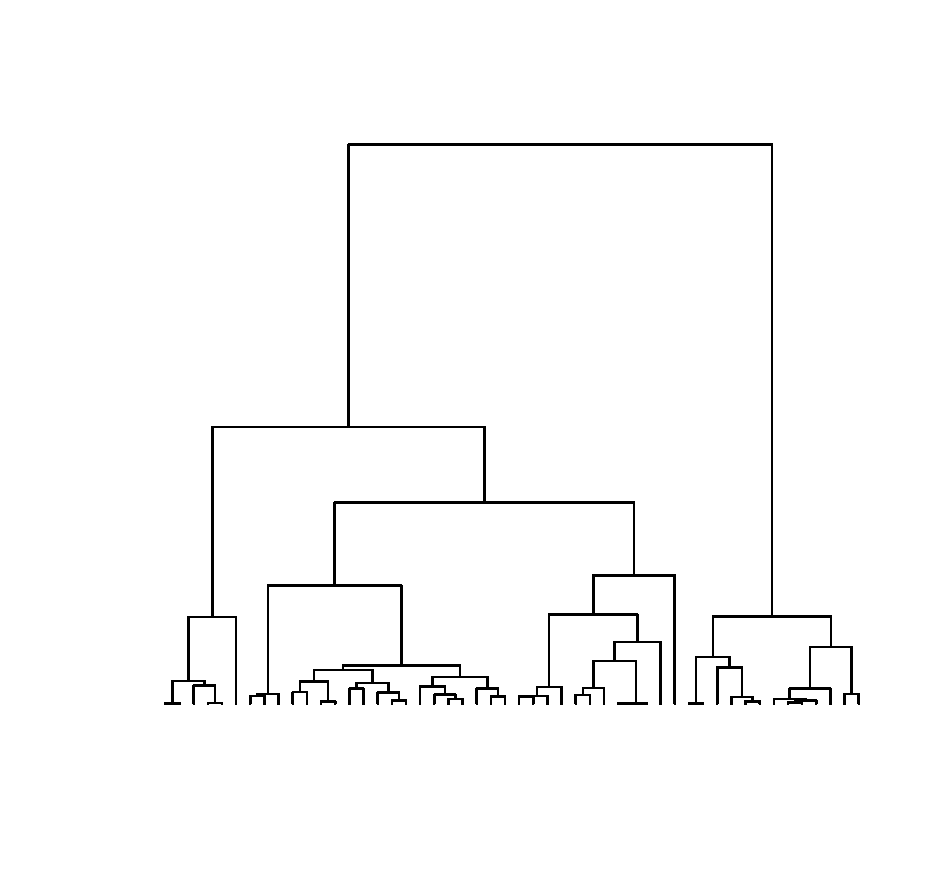
\includegraphics[width=\textwidth, trim={2.8cm 3cm 1.5cm 2cm}, clip]{ncoalescent.pdf}
\end{column}
\end{columns}
\end{frame}


\begin{frame}{Scenario}
\begin{itemize}
\item Population size $N$
\item Discrete generations
\item Sample $n \leq N$ individuals from the terminal generation
\item Rescale time appropriately
\item Let $N\to\infty$
\end{itemize}
\end{frame}


\begin{frame}{Sufficient conditions, neutral case}
\begin{theorem}[Kingman 1982]
\begin{itemize}
\item Individuals are exchangeable
\item Offspring counts $\nu^{(1:N)}$ are i.i.d. across generations
\item $\V[ \nu^{(1)} ] = \sigma_N^2 \longrightarrow \sigma^2 \in (0,\infty)$
\item $\sup_N \E[ (\nu^{(1)})^k] <\infty$ for all $k\geq 3$
\end{itemize}
Then the rescaled genealogy of $n$ individuals converges weakly to the $n$-coalescent as $N\to\infty$.
\end{theorem}
\end{frame}


\begin{frame}{Sufficient conditions, neutral case}
\begin{itemize}
\item Exchangeability = neutrality (genotype does not affect number of offspring)
\pause
\item System completely specified by distribution of $\nu^{(1:N)}$
\item \textbf{Wright-Fisher model:} $\nu^{(1:N)} \sim \Mn( N, (\frac{1}{N},\dots, \frac{1}{N}) )$
\item \textbf{Moran model:} $\nu^{(1:N)}$ uniform over permutations of $(2,0,1,\dots, 1)$
\pause
\item Since $\sum \nu^{(i)} = N$ and individuals are exchangeable, $\E[\nu^{(i)}] = 1$.
\item Case $\sigma^2 = 0$ would mean no coalescences in the limit
\end{itemize}
\end{frame}


\begin{frame}{Necessary and sufficient conditions, neutral case}
\begin{theorem}[M\"ohle Sagitov 2001, 2003]
\begin{itemize}
\item Individuals are exchangeable
\item Offspring counts $\nu^{(1:N)}$ are i.i.d. across generations
\item $c_N >0$ for all $N<\infty$
\item $c_N \longrightarrow 0$
\item $d_N/c_N \longrightarrow 0$
\end{itemize}
If and only if the rescaled genealogy of $n$ individuals converges weakly to the $n$-coalescent as $N\to\infty$.
\end{theorem}
\begin{equation*}
d_N := \frac{N \E[ ( \nu^{(1)} )_3 ] }{(N)_3}  ,\qquad
c_N := \frac{N \E[ ( \nu^{(1)} )_2 ] }{(N)_2} 
\end{equation*}
\end{frame}


\begin{frame}{Necessary and sufficient conditions, neutral case}
\begin{itemize}
\item The condition $c_N >0$ plays the same role as Kingman's condition $\sigma^2 >0$
\item $c_N = \frac{\V[\nu^{(1)}]}{N-1}$, so $c_N \to 0$ is weaker than Kingman's condition $\V[ \nu^{(1)} ] \to \sigma^2$
\item Only requires control up to 3rd moment, cf.\ Kingman requires \emph{all} moments finite
\end{itemize}
\end{frame}


\begin{frame}{Sufficient conditions, non-neutral case}
\begin{theorem}[B Koskela Jenkins Johansen 2021]
\begin{itemize}
\item Given $\nu_t^{(1:N)}$, assignment of offspring to parents is uniform over all valid assignments
\item Time scale is almost surely finite
\item $\exists$ deterministic sequence $b_N \to 0$ such that $\forall N, t$
\begin{equation*}
\frac{1}{(N)_3} \sum_{i=1}^N \E_t[ (\nu_t^{(i)})_3 ]
\leq b_N \frac{1}{(N)_2} \sum_{i=1}^N \E_t[ (\nu_t^{(i)})_2 ]
\end{equation*}
\end{itemize}
Then the rescaled genealogy of $n$ individuals converges weakly to the $n$-coalescent as $N\to\infty$.
\end{theorem}
\end{frame}


%\begin{frame}{Sufficient conditions, non-neutral case}
%\begin{itemize}
%\item Not exchangeable, so individual index kept explicit
%\item Not i.i.d. over time, so $t$ kept explicit, and time scale is not constant!
%\item The finite time scale condition plays the same role as Kingman's $\sigma^2>0$ 
%\item The main condition is the non-exchangeable analogue of M\"ohle \& Sagitov's $d_N/c_N \to 0$
%\item Verified for several systems of interest in sequential Monte Carlo
%\end{itemize}
%\end{frame}


%\begin{frame}{In conclusion...}
%\begin{itemize}
%\item ?
%\end{itemize}
%\end{frame}

\begin{frame}{Open questions}
\begin{itemize}
\item Are the conditions necessary and sufficient in the non-neutral case?
\item What does the random time scale look like?
\item Rate of convergence?
\item Can the conditions be verified for some interesting population genetic models?
\end{itemize}
\end{frame}


\begin{frame}{References}
\begin{enumerate}
\item JFC Kingman (1982) \textit{The coalescent}. Stochastic Processes and Their Applications 13:235--248.
\item JFC Kingman (1982) \textit{On the genealogy of large populations}. Journal of Applied Probability 19A:27--43.
\item M M\"ohle, S Sagitov (2001) \textit{A classification of coalescent processes for haploid exchangeable population models}. The Annals of Probability 29(4):1547--1562.
\item M M\"ohle, S Sagitov (2003) \textit{Coalescent patterns in diploid exchangeable population models}. Journal of Mathematical Biology 47(4):337--352.
\item S Brown, PA Jenkins, AM Johansen, J Koskela (2021) \textit{Simple conditions for convergence of sequential Monte Carlo genealogies with applications}. Electronic Journal of Probability 26:1--22.
\end{enumerate}
\end{frame}

\end{document}